\section{Метод конечных разностей для решения одномерного нестационарного уравнения диффузии}
\subsection{Коэффициент диффузии не зависит от концентрации}
Одномерное нестационарное уравнение диффузии, соответствующее второму закону Фика имеет вид:
\begin{equation}\label{eq:difft}
	\frac{\delta}{\delta t} C = D\frac{\delta^{2}}{\delta x^2} C;
\end{equation}

Аппроксимация первой производной по времени в момент времени $t_{i}$ концентрации $C_{j}(t_{i}) = C^{i}_{j}$ в точке $j$:
\begin{equation}\label{eq:diffdt1}
	\frac{\delta}{\delta t} C^{i}_{j} = \frac{C^{i+1}_{j} - C^{i}_{j}}{\Delta t};
\end{equation}

Аппроксимация первой производной по координате в момент времени $t_{i}$ концентрации $C_{j}(t_{i}) = C^{i}_{j}$ в точке $j$:
\begin{equation}\label{eq:diffdx1}
	J^{i}_{j} = \frac{\delta}{\delta x} C^{i}_{j} = \frac{C^{i}_{j+1} - C^{i}_{j}}{\Delta x};
\end{equation}

Аппроксимация второй производной по координате в момент времени $t_{i}$ концентрации $C_{j}(t_{i}) = C^{i}_{j}$ в точке $j$:
\begin{equation*}
	\frac{\delta^{2}}{\delta x^{2}} C^{i}_{j} = \frac{\delta}{\delta x}\bigg[ \frac{C^{i}_{j+1} - C^{i}_{j}}{\Delta x} \bigg] = \frac{ \frac{C^{i}_{j+1} - C^{i}_{j}}{\Delta x} - \frac{C^{i}_{j} - C^{i}_{j-1}}{\Delta x}}{\Delta x} = 
\end{equation*}
\begin{equation}\label{eq:diffdx2}
	= \frac{C^{i}_{j+1} - 2C^{i}_{j} + C^{i}_{j-1}}{\Delta x^2};
\end{equation}

Подставляя в (\ref{eq:difft}) аппроксимацию производных (\ref{eq:diffdt1}), (\ref{eq:diffdx2}), получим связь $C^{i+1}_{j}$ с $C^{i}_{j}$, т.е. изменение концентрации через $\Delta t$:

\begin{equation}\label{eq:diffFD}
	C^{i+1}_{j} = \lambda C^{i}_{j-1} + (1 - 2\lambda)C^{i}_{j} + \lambda C^{i}_{j+1},
\end{equation}
где $\lambda = \frac{D\Delta t}{\Delta x^2}$~---  связь коэффициента диффузии и шагов по сетке времени и координаты.

Уравнение (\ref{eq:diffFD}) справедливо для всех не крайних точек конечно разностной схемы, при коэффициенте диффузии не зависящем от концентрации.

Выделим два граничных приближения для концентрации:
\begin{enumerate}
	\item <<Закрытая система>> ~--- концентрация на границе не изменяется ($J_{0}^{i} = 0$, $J_{N+1}^{i} = 0$), см. рис.\ref{fig:DS}, а);
	\item <<Открытая система>> ~--- поток частиц подходящий к границе равен потоку уходящих частиц ($J_{0}^{i} = J_{1}^{i}$, $J_{N}^{i} = J_{N+1}^{i}$), см. рис.\ref{fig:DS}, б).
\end{enumerate}

\noindent
\begin{minipage}{0.4\textwidth}
	\centering
	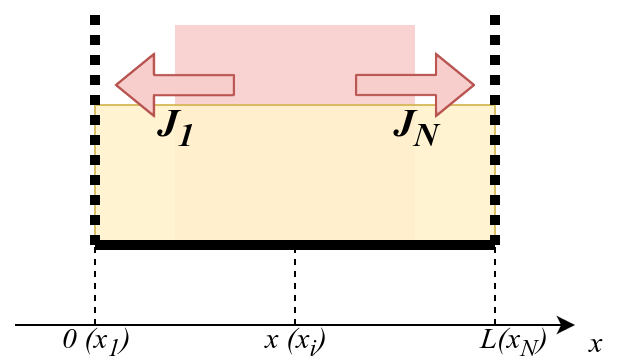
\includegraphics[width=\linewidth]{assets/CD}
	а)
\end{minipage}
~
\begin{minipage}{0.6\textwidth}
	\centering
	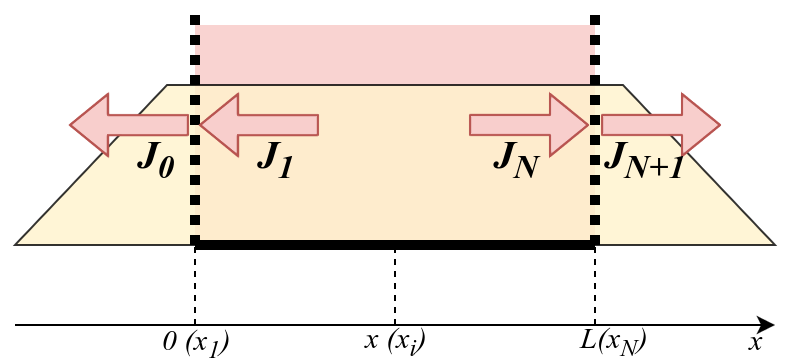
\includegraphics[width=\linewidth]{assets/OD}
	б)
\end{minipage}
\begin{figure}
	\centering
	% 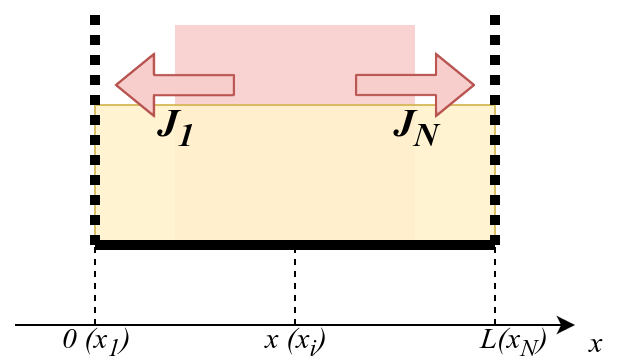
\includegraphics[width=0.9\linewidth]{assets/CD}
	\caption{a) <<Закрытая>>, б) <<Открытая>> система диффузии}
	\label{fig:DS}
\end{figure}

Для <<закрытой системы>> должно выполняться условие $J_{0}^{i} = 0$, $J_{N+1}^{i} = 0$. Рассмотрим (\ref{eq:diffdx1}), (\ref{eq:diffFD}) для точки $j = 1$:
\begin{gather*}
 	J^{i}_{0} = \frac{C^{i}_{1} - C^{i}_{0}}{\Delta x} = 0 \Rightarrow C_{0}^{i} = C_{1}^{i};\\
	C^{i+1}_{1} = \lambda C^{i}_{0} + (1 - 2\lambda)C^{i}_{1} + \lambda C^{i}_{2} = \lambda C^{i}_{1} + (1 - 2\lambda)C^{i}_{1} + \lambda C^{i}_{2} = \\
	= (1 - \lambda)C^{i}_{1} + \lambda C^{i}_{2} = C^{i+1}_{1};
\end{gather*}

Рассматривая точки $N-1$, $N$, $N+1$ аналогичным образом получим:

\begin{equation}
	\label{eq:CD}
	\begin{cases}
		C^{i+1}_{1} = (1 - \lambda)C^{i}_{1} + \lambda C^{i}_{2};\\
		C^{i+1}_{j} = \lambda C^{i}_{j-1} + (1 - 2\lambda)C^{i}_{j} + \lambda C^{i}_{j+1},\,j \in [2,\,\dots,\,N-1];\\
		C^{i+1}_{N} = (1 - \lambda)C^{i}_{N} + \lambda C^{i}_{N-1};\\
		\lambda = D\frac{\Delta t}{\Delta x^{2}}.
	\end{cases}
\end{equation}

Для решения системы уравнений (\ref{eq:CD}) в среде \textsc{MatLab} была составлена функция \texttt{getDiffCloseAlGaAs} (лист. \ref{lst:CD}). С помошью данной функции мы сможем моделировать диффузионное расплытие атомов $Al$ в <<закрытой>> гетероструктуре на основе $i$-$Al_{x}Ga_{1-x}As$.

Входыне параметры функции: профиль доли содержания $Al$ в $Al_{x}Ga_{1-x}As$, массив времени, через которое необходимо получить профиль деградированной структуры, шаг сетки и температура системы. Выходынми данными являются: Профиль дна зоны проводимости, профиль эффективной массы элеткронов в зоне проводимости, профиль доли доли содержания $Al$ в $i$-$Al_{x}Ga_{1-x}As$.
\begin{lstlisting}[style=realcode,language=Matlab,caption={Функция рассчета диффузионного расплытия $Al$ в <<закрытой>> гетероструктуре на основе $i$-$Al_{x}Ga_{1-x}As$},label={lst:CD}]
function [Ec, meff, Alx] = getDiffCloseAlGaAs(x_Al, checkTime, dx, T)
	e = 1.6e-19; eVtoJ = e; JtoEv = e^(-1);
	nm = 1e-9; me = 9.1*1e-31;
	hbar = 1.054*1e-34; k_B = 1.38e-23;

	kT = T*k_B; % J

	Time = max(checkTime)*12*30*24; % to hours

	n_Atoms = 4.42*1e28; % number Atoms in GaAs ~ AlAs
	n_Al = n_Atoms/2; % number atoms of Al in AlAs

	dt = 1; % one hour
	dtdx2 = dt*60*60/dx^2; % s/m^2

	D_Al = 0.2*exp(-3.5/(kT*JtoEv))*1e-4; % m^2/s

	C_Al = x_Al*n_Al;
	len = length(x_Al);

	d1 = D_Al*dtdx2*ones(1, len-1);
	d2 = [ 1 - D_Al*dtdx2, 1 - 2*D_Al*dtdx2*ones(1, len-2), 1 - D_Al*dtdx2 ];
	d3 = D_Al*dtdx2*ones(1, len-1);
	
	Matrix_Al = diag(d1, -1) + diag(d2) + diag(d3, +1);

	if (find(0 == checkTime))
		[Ec(1, :), ~, meff(1, :), ~] = getBandPropAlGaAs(C_Al);
		Alx(1, :) = C_Al./n_Al;		
	end

	C_Al = C_Al';
	for j = 0 : dt : Time
		C_Al = Matrix_Al*C_Al;
		ind = find(j == checkTime*12*30*24); 
		if (ind & j ~= 0)
			[Ec(ind, :), ~, meff(ind, :), ~] = getBandPropAlGaAs(C_Al');
			Alx(ind, :) = C_Al'./n_Al;
		end
	end
end
\end{lstlisting}

В строке 2 задаются: заряд электрона и константы перевода из эВ в Дж и наоборот. В строке 3 задаются константа перевода и метров в нанометры и масса покоя электрона. В строке 4 задаются постоянная Дирака и константа Больцмана.

В строке 8 массив годов проверки переводится в массив часов. В строках 10, 11 задается количество частиц в кубическом сантиметре $GaAs$ и количество атомов $Al$ в $AlAs$. Количество частиц в $AlAs$ и $GaAs$ практически одинаковое. В строках 13, 14 задается шаг сетки по врени, в данном случае 1 час, и задается велечина $\frac{\Delta t}{\Delta x^{2}}$ в СИ.

В строке 16 задается коэффициент диффузии. В строке 18 задаются начальыне условия -- концентрация атомов $Al$ в $i$-$Al_{x}Ga_{1-x}As$. В строке 22 задается конечно-разностная схема для внутренних точек гетероструктуры. В строках 21, 23 задаются граничные условия, в соответствии с (\ref{eq:CD}). В строке 25 создается матрица, удовлетворяющая системе (\ref{eq:CD}). В строках 33-40 рассчитывается диффузионное расплытие под действием гардиента концентрации при фиксированной температуре.

С помощью лист.~\ref{lst:mainDiff} (см. прил.~\ref{app:Diff}) можно рассчитать процесс диффузии $Al$ под действием градиента концентрации при фиксированной температуре из $i$-$AlAs$ в $i$-$GaAs$ в закрытой системе представленной на рис.~\ref{fig:DCloseBox}.
\begin{figure}[h!]
	\centering
	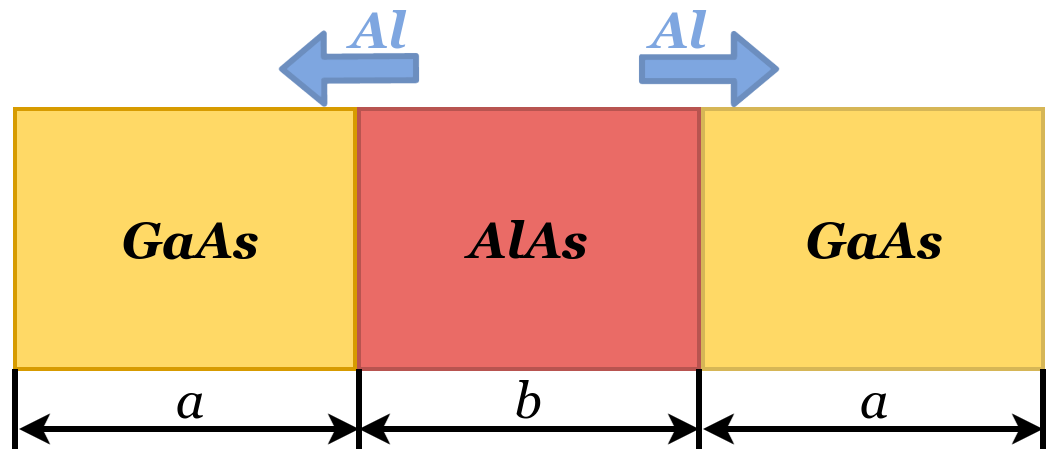
\includegraphics[width=0.9\linewidth]{assets/DCloseBox}
	\caption{Графическая схема <<закрытой>> гетероструктуры $GaAs$/$AlAs$/$GaAs$}
	\label{fig:DCloseBox}
\end{figure}

В закрытой системе атомы $Al$ не могу покинуть пределы системы, поэтому на краях гетероструктур со временем будут накапливаться атомы $Al$. Параметры исследуемой модели (см. рис.~\ref{fig:DCloseBox}):
\begin{itemize}
	\item $a = 10$ монослоев;
	\item $b = 30$ монослоев;
	\item Температура $T = 920\,K$;
	\item Время деградации $[1,\,2,\,3,\,4,\,5]$ лет.
\end{itemize}
Результат моделирования представлена на рис.~\ref{fig:DCAl}. Атомы $Al$ не уходят за границу исследуемой гетероструктуры.

\begin{figure}[h!]
	\centering
	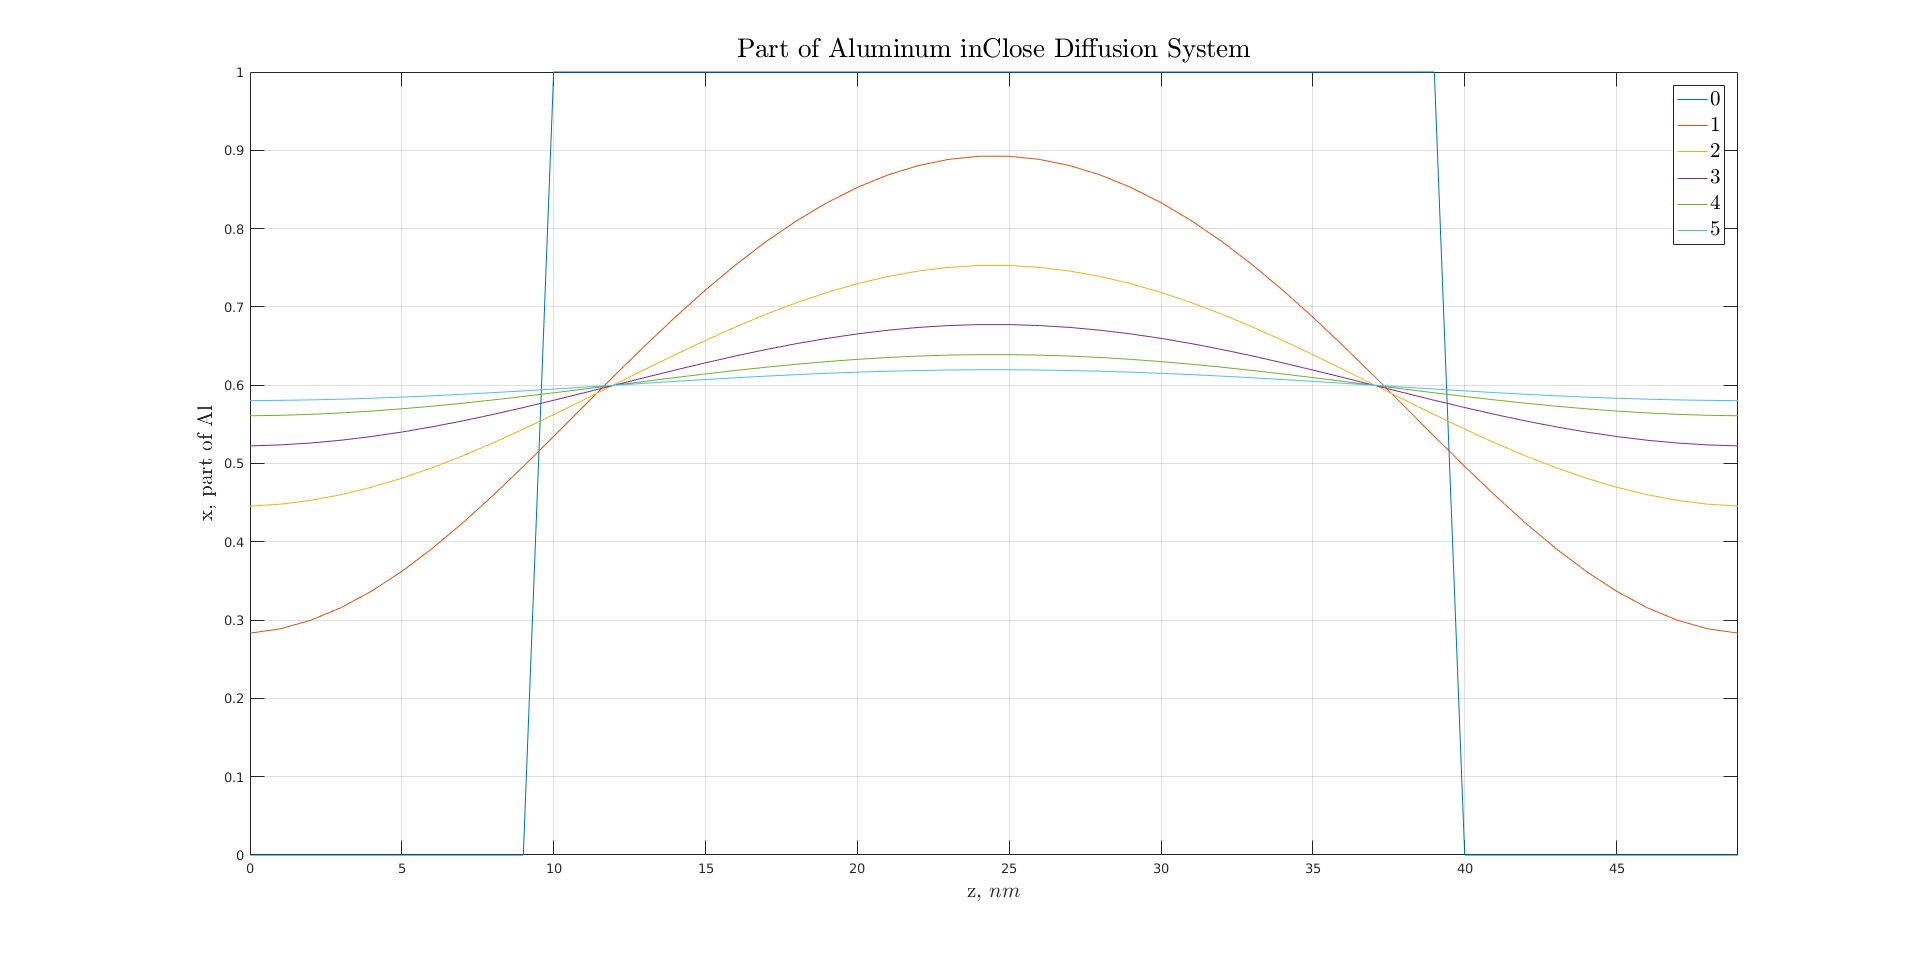
\includegraphics[width=0.9\linewidth]{assets/DCAl}
	\caption{Диффузионное расплытие <<закрытой>> гетероструктуры $i$-$GaAs$/$i$-$AlAs$/$i$-$GaAs$ при $T = 920\,K$}
	\label{fig:DCAl}
\end{figure}

Для <<открытой>> системы должно выполняться условие $J_{0}^{i} = J_{1}^{i}$, $J_{N}^{i} = J_{N+1}^{i}$. Рассмотрим (\ref{eq:diffdx1}), (\ref{eq:diffdx2}), (\ref{eq:diffFD}) для точки $j = 1$:

\begin{gather*}
 	J^{i}_{0} = J^{i}_{1}\\
	\frac{C^{i+1}_{1} - C^{i}_{1}}{\Delta t} = \frac{J^{i}_{1} - J^{i}_{0}}{\Delta x} = \frac{0}{\Delta x} = 0\Rightarrow\\
	\Rightarrow C^{i+1}_{1} = C^{i}_{1};
\end{gather*}

Рассматривая точки $N-1$, $N$, $N+1$ аналогичным образом получим:

\begin{equation}
	\label{eq:DDiffConst}
	\begin{cases}
		C^{i+1}_{1} = C^{i}_{1};\\
		C^{i+1}_{j} = \lambda C^{i}_{j-1} + (1 - 2\lambda)C^{i}_{j} + \lambda C^{i}_{j+1},\,j \in [2,\,\dots,\,N-1];\\
		C^{i+1}_{N} = C^{i}_{N};\\
		\lambda = D\frac{\Delta t}{\Delta x^{2}}.
	\end{cases}
\end{equation}

Для решения системы уравнений (\ref{eq:DDiffConst}) в среде \textsc{MatLab} была составлена функция \texttt{getDiffOpenAlGaAs} (лист. \ref{lst:OD}). С помошью данной функции мы сможем моделировать диффузионное расплытие атомов $Al$ в <<открытой>> гетероструктуре на основе $i$-$Al_{x}Ga_{1-x}As$.

Входыне параметры функции: профиль доли содержания $Al$ в $Al_{x}Ga_{1-x}As$, массив времени, через которое необходимо получить профиль деградированной структуры, шаг сетки и температура системы. Выходынми данными являются: Профиль дна зоны проводимости, профиль эффективной массы элеткронов в зоне проводимости, профиль доли доли содержания $Al$ в $i$-$Al_{x}Ga_{1-x}As$.

\begin{lstlisting}[style=realcode,language=Matlab,caption={Функция расчета диффузионного расплытия атомов $Al$ в <<открытой>> системе $i$-$Al_{x}Ga_{1-x}As$},label={lst:OD}]
function [Ec, meff, Alx] = getDiffOpenAlGaAs(x_Al, checkTime, dx, T)
	e = 1.6e-19; eVtoJ = e; JtoEv = e^(-1);
	nm = 1e-9; me = 9.1*1e-31;
	hbar = 1.054*1e-34; k_B = 1.38e-23;

	kT = T*k_B; % J
	
	Time = max(checkTime)*12*30*24; % to hours
	
	n_Atoms = 4.42*1e28; % number Atoms in GaAs ~ AlAs
	n_Al = n_Atoms/2; % number atoms of Al in AlAs

	dt = 1; % one hour
	dtdx2 = dt*60*60/dx^2; % s/m^2

	D_Al = 0.2*exp(-3.5/(kT*JtoEv))*1e-4; % m^2/s

	C_Al = x_Al*n_Al;
	len = length(x_Al);

	d1 = [D_Al*dtdx2*ones(1, len-2), 0];
	d2 = [ 1, 1 - 2*D_Al*dtdx2*ones(1, len-2), 1 ];
	d3 = [0, D_Al*dtdx2*ones(1, len-2)];
	
	Matrix_Al = diag(d1, -1) + diag(d2) + diag(d3, +1);

	if (find(0 == checkTime))
		[Ec(1, :), ~, meff(1, :), ~] = getBandPropAlGaAs(C_Al);
		Alx(1, :) = C_Al./n_Al;		
	end

	C_Al = C_Al';
	for j = 0 : dt : Time
		C_Al = Matrix_Al*C_Al;
		ind = find(j == checkTime*12*30*24); 
		if (ind & j ~= 0)
			[Ec(ind, :), ~, meff(ind, :), ~] = getBandPropAlGaAs(C_Al');
			Alx(ind, :) = C_Al'./n_Al;
		end
	end
end
\end{lstlisting}
В строке 2 задаются: заряд электрона и константы перевода из эВ в Дж и наоборот. В строке 3 задаются константа перевода и метров в нанометры и масса покоя электрона. В строке 4 задаются постоянная Дирака и константа Больцмана.

В строке 8 массив годов проверки переводится в массив часов. В строках 10, 11 задается количество частиц в кубическом сантиметре $GaAs$ и количество атомов $Al$ в $AlAs$. Количество частиц в $AlAs$ и $GaAs$ практически одинаковое. В строках 13, 14 задается шаг сетки по врени, в данном случае 1 час, и задается велечина $\frac{\Delta t}{\Delta x^{2}}$ в СИ.

В строке 16 задается коэффициент диффузии. В строке 18 задаются начальыне условия -- концентрация атомов $Al$ в $i$-$Al_{x}Ga_{1-x}As$. В строке 22 задается конечно-разностная схема для внутренних точек гетероструктуры. В строках 21, 23 задаются граничные условия, в соответствии с (\ref{eq:DDiffConst}). В строке 25 создается матрица, удовлетворяющая системе (\ref{eq:DDiffConst}). В строках 33-40 рассчитывается диффузионное расплытие под действием гардиента концентрации при фиксированной температуре.

С помощью лист.~\ref{lst:mainDiff} (см. прил.~\ref{app:Diff}) можно рассчитать процесс диффузии $Al$ под действием градиента концентрации при фиксированной температуре из $i$-$AlAs$ в $i$-$GaAs$ в открытой системе представленной на рис.~\ref{fig:DOpeneBox}.
\begin{figure}[h!]
	\centering
	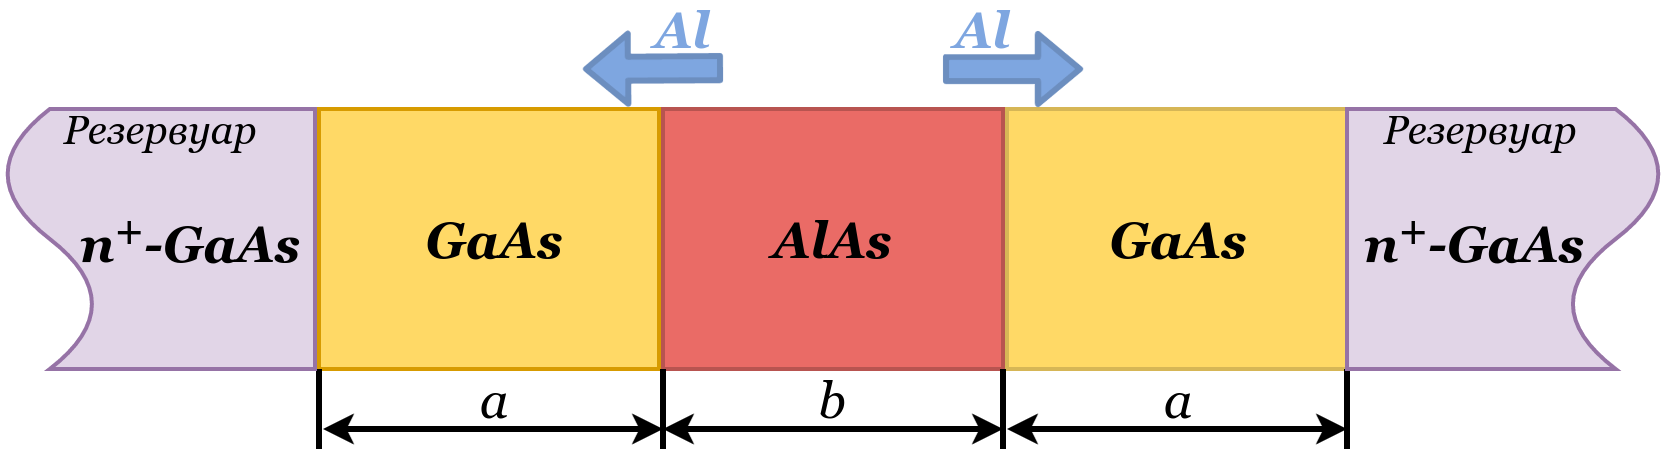
\includegraphics[width=0.9\linewidth]{assets/DOpenBox}
	\caption{Графическая схема <<открытой>> гетероструктуры $GaAs$/$AlAs$/$GaAs$}
	\label{fig:DOpeneBox}
\end{figure}

Предположим, что в рассматриваемой системе (рис.~\ref{fig:DOpeneBox}) атомы $Al$, достигнув резервуаров покидают исследуемую гетероструктуру (не будем рассматривать резервуары, как часть исследуемой системы). Так же предположим, что скорость ухода частиц $Al$ быстрее, чем их подход. Параметры исследуемой модели (см. рис.~\ref{fig:DOpeneBox}):
\begin{itemize}
	\item $a = 10$ монослоев;
	\item $b = 30$ монослоев;
	\item Температура $T = 920\,K$;
	\item Время деградации $[1,\,2,\,3,\,4,\,5]$ лет.
\end{itemize}
Результат моделирования представлена на рис.~\ref{fig:DOAl}. Атомы $Al$ покидают исследуемую гетероструктуру и общая концентрация $Al$ в гетероструктуре снижается.

\begin{figure}[h!]
	\centering
	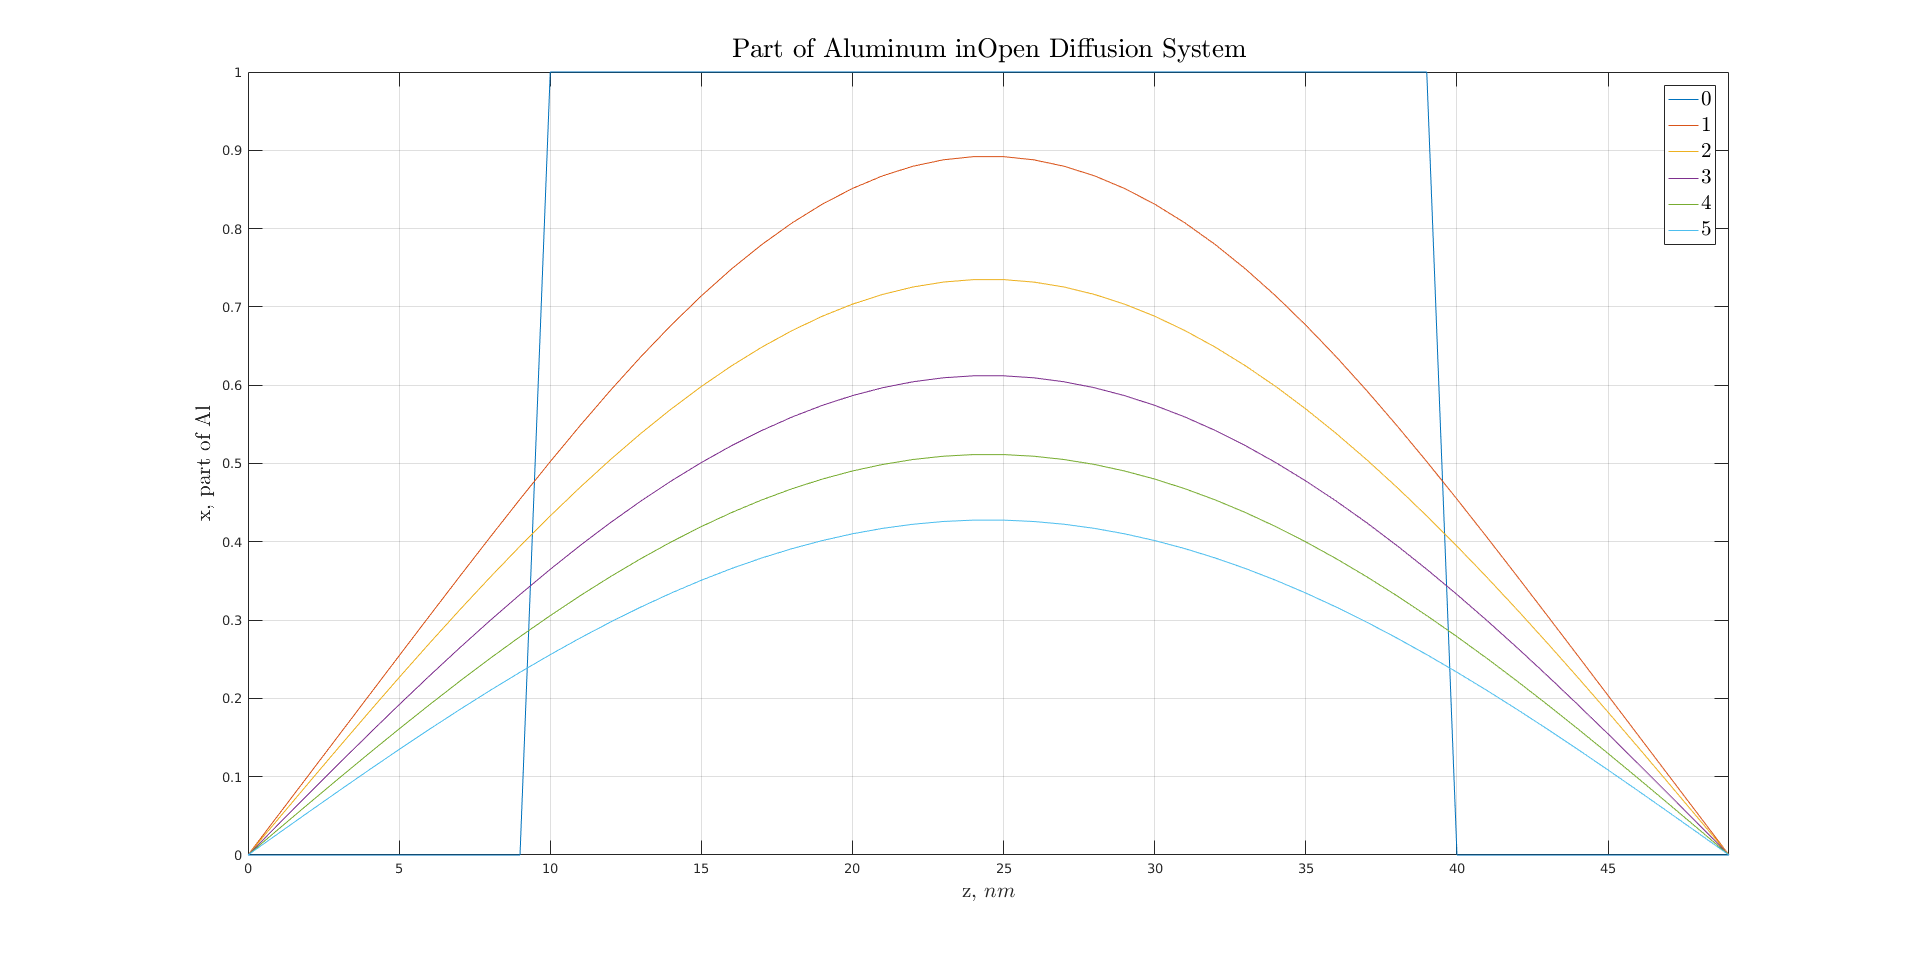
\includegraphics[width=0.9\linewidth]{assets/DOAl}
	\caption{Диффузионное расплытие <<закрытой>> гетероструктуры $i$-$GaAs$/$i$-$AlAs$/$i$-$GaAs$ при $T = 920\,K$}
	\label{fig:DOAl}
\end{figure}

\subsection{Коэффициент диффузии зависит от концентрации}

Если коэффициенте диффузии (D) зависит от концентрации, тогда уравнение диффузии принимает вид:

\begin{equation}\label{eq:diffD(x)t}
	\frac{\delta}{\delta t} C = \frac{\delta}{\delta x}D\frac{\delta}{\delta x} C;
\end{equation}

Тогда уравнение конечно-разностной схемы будет~\cite{FDDiff}:

\begin{gather}\label{eq:diffD(x)tFD}
	\frac{C_{j}^{i+1} - C_{j}^{i}}{\Delta t} = \frac{ D_{j+1/2}^{i}\frac{C^{i}_{j+1} - C^{i}_{j}}{\Delta x} - D_{j-1/2}^{i}\frac{C^{i}_{j} - C^{i}_{j-1}}{\Delta x} }{\Delta x};\\
	D_{j\pm1/2}^{i} = \frac{D^{i}_{j} + D^{i}_{j\pm1}}{2} = D_{j\pm}^{i}.
\end{gather}

Проводя рассуждения аналогичные предыдущему параграфу получит конечно-разностную схему для открытой схемы:

\begin{equation}
	\label{eq:DFromC}
	\begin{cases}
		C^{i+1}_{1} = C^{i}_{1};\\
		C^{i+1}_{j} = \lambda_{-}^{i} C^{i}_{j-1} + (1 - \lambda^{i}_{+} - \lambda^{i}_{-})C^{i}_{j} + \lambda^{i}_{+} C^{i}_{j+1},\,j \in [2,\,\dots,\,N-1];\\
		C^{i+1}_{N} = C^{i}_{N};\\
		\lambda^{i}_{+} = D_{j+}^{i}\frac{\Delta t}{\Delta x^{2}};\\
		\lambda^{i}_{-} = D_{j-}^{i}\frac{\Delta t}{\Delta x^{2}}.
	\end{cases}
\end{equation}

Для решения системы (\ref{eq:DFromC}) в среде \textsc{MatLab} была реализована функция \texttt{getDiffAlGaAs\_Si} (лист.\ref{lst:DFromC}). Данная функция рассчитывает диффузионное расплытие атомов $Al$ в гетероструктуре на основе $Al_{x}Ga_{1-x}As$ под действием градиента концентрации при фиксированной температуре, с учетом проникновения легирующей примеси $Si$.

Входыне параметры функции: профиль доли содержания $Al$ в $Al_{x}Ga_{1-x}As$, массив времени, через которое необходимо получить профиль деградированной структуры, шаг сетки и температура системы, концетрация легирующей примеси на границе гетероструктуры. Выходынми данными являются: Профиль дна зоны проводимости, профиль эффективной массы элеткронов в зоне проводимости, профиль доли доли содержания $Al$ в $i$-$Al_{x}Ga_{1-x}As$, доля содержания атомов примеси ($Si$) в гетероструктуре.
\begin{lstlisting}[style=realcode,language=Matlab,caption={Функция расчета диффузионного расплытия атомов $Al$ в <<открытой>> системе $i$-$Al_{x}Ga_{1-x}As$ с учетом коэффициента диффузии, зависящего от концентрации легирующей примеси},label={lst:DFromC}]
function [Ec, meff, Alx, Six] = getDiffAlGaAs_Si(x_Al, checkTime, dx, T, n_Si)
	e = 1.6e-19; eVtoJ = e; JtoEv = e^(-1);
	nm = 1e-9; me = 9.1*1e-31;
	hbar = 1.054*1e-34; k_B = 1.38e-23;

	kT = T*k_B; % J

	Time = max(checkTime)*12*30*24; % to hours

	n_Atoms = 4.42*1e28; % number Atoms in GaAs ~ AlAs
	n_Al = n_Atoms/2; % number atoms of Al in AlAs

	dt = 1; % one hour
	dtdx2 = dt*60*60/dx^2; % s/m^2

	Eg_GaAs = 1.519 - 5.405*1e-4*T^2/(T+204);
	Nc = 2*(me*0.067*kT/pi/hbar^2/2)^(3/2);
	Nv = 2*(me*0.51*kT/pi/hbar^2/2)^(3/2);
	ni = sqrt(Nc*Nv)*exp(-Eg_GaAs/(2*kT*JtoEv));

	C_Al = [0, x_Al, 0]*n_Al;
	len = length(C_Al);

	C_Si = [n_Si, ni*ones(size(x_Al)), n_Si];

	if (find(0 == checkTime))
		[Ec(1, :), ~, meff(1, :), ~] = getBandPropAlGaAs(C_Al(2:end-1));
		Alx(1, :) = C_Al(2:end-1)./n_Al;		
		Six(1, :) = C_Si(2:end-1)./n_Si;		
	end

	C_Al = C_Al';
	C_Si = C_Si';
	for j = 0 : dt : Time
		D = 0.2*exp(-3.5/(kT*JtoEv))*(C_Si'./ni).^3*1e-4;

		D_plus = (D(1:len-1) + D(2:len))./2;
		D_minus = (D(2:len) + D(1:len-1))./2;

		d1 = [D_minus(1:end-1)*dtdx2, 0];
		d2 = [1, 1 - (D_plus(2:end) + D_minus(1:end-1))*dtdx2, 1];
		d3 = [0, D_plus(2:end)*dtdx2];
		Matrix = diag(d1, -1) + diag(d2) + diag(d3, +1);

		C_Al = Matrix*C_Al;
		C_Si = Matrix*C_Si;

		ind = find(j == checkTime*12*30*24); 
		if (ind & j ~= 0)
			[Ec(ind, :), ~, meff(ind, :), ~] = getBandPropAlGaAs(C_Al(2:end-1)');
			Alx(ind, :) = C_Al(2:end-1)'./n_Al;
			Six(ind, :) = C_Si(2:end-1)';
		end
	end
end
\end{lstlisting}
В строке 2 задаются: заряд электрона и константы перевода из эВ в Дж и наоборот. В строке 3 задаются константа перевода и метров в нанометры и масса покоя электрона. В строке 4 задаются постоянная Дирака и константа Больцмана.

В строке 8 массив годов проверки переводится в массив часов. В строках 10, 11 задается количество частиц в кубическом сантиметре $GaAs$ и количество атомов $Al$ в $AlAs$. Количество частиц в $AlAs$ и $GaAs$ практически одинаковое. В строках 13, 14 задается шаг сетки по врени, в данном случае 1 час, и задается велечина $\frac{\Delta t}{\Delta x^{2}}$ в СИ.

В строках 16-19 рассчитывается концентрация собственных носителей заряда и в случаи чистого полупроводника приравнивается к концентрации донорной примеси. В строках 21, 24 задаются начальные условия -- профиль концентрации $Al$ и $Si$. Строки 32, 33 преобразуют строку в столбец, для преобразования. 

В строках 24-34 рассчитывается диффузионное расплытие гетероструктуры. Цикл выполняется с шагом сетки по времени. В строке 35 каждый цикл пересчитывается коэффициент диффузии, так как изменяется концентрация $Al$ и $Si$. В строках 37, 38 рассчитываются средние значения коэффициента диффузии, в соответствии с коненчо-разностной схемой (\ref{eq:DFromC}). В строке 41 объявляется конечно-разностная схема для внутрненних точек гетероструктуры. В строках 40, 42 объявляются граничные условия. В строках 43, 45, 46 объявляется матрица преобразования и происходит расчет диффузии атомов $Al$ и $Si$ в гетероструктуре.

С помощью лист.~\ref{lst:mainDiff} (см. прил.~\ref{app:Diff}) можно рассчитать процесс диффузии $Al$ под действием градиента концентрации при фиксированной температуре из $i$-$AlAs$ в $i$-$GaAs$ с учетом диффузии легирующей примеси из резервуаров на схеме представленной на рис.~\ref{fig:DSiBox}.
\begin{figure}[h!]
	\centering
	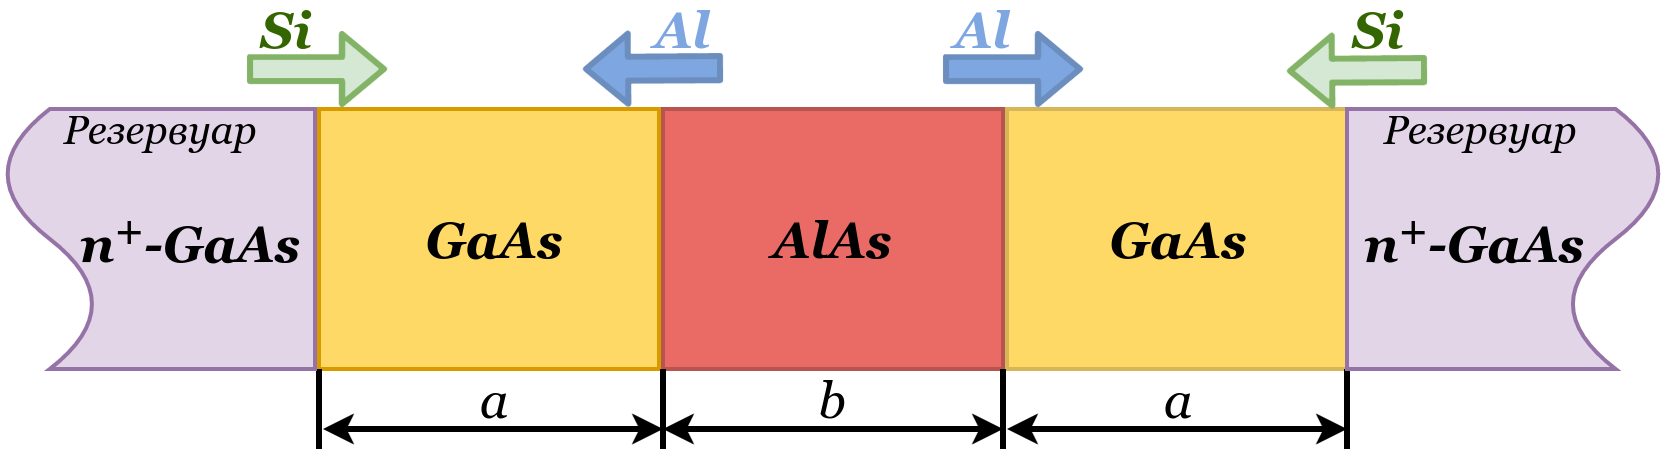
\includegraphics[width=0.8\linewidth]{assets/DSiBox}
	\caption{Графическая схема гетероструктуры $GaAs$/$AlAs$/$GaAs$ с диффундирующими атомами $Al$ и $Si$}
	\label{fig:DSiBox}
\end{figure}

Проникновение легирующей примеси увеличивает коэффициент диффузии и скорость термической деградации гетероструктуры в соответствии с (\ref{eq:DNd}). Параметры исследуемой модели (см. рис.~\ref{fig:DSiBox}):
\begin{itemize}
	\item $a = 10$ монослоев;
	\item $b = 30$ монослоев;
	\item Концентрация донорной примеси $N_{D} = 10^{24}\,m^{-3}$;
	\item Температура $T = 430\,K$;
	\item Время деградации $[1,\,2,\,3,\,4,\,5]$ лет.
\end{itemize}
Результат моделирования представлена на рис.~\ref{fig:DSi}. С уменьшением температуры факторов, влияющим на диффузию атомов $Al$ стала глубина проникновения атомов легирующей примеси ($Si$) из резервуаров.

\begin{figure}[h!]
	\centering
	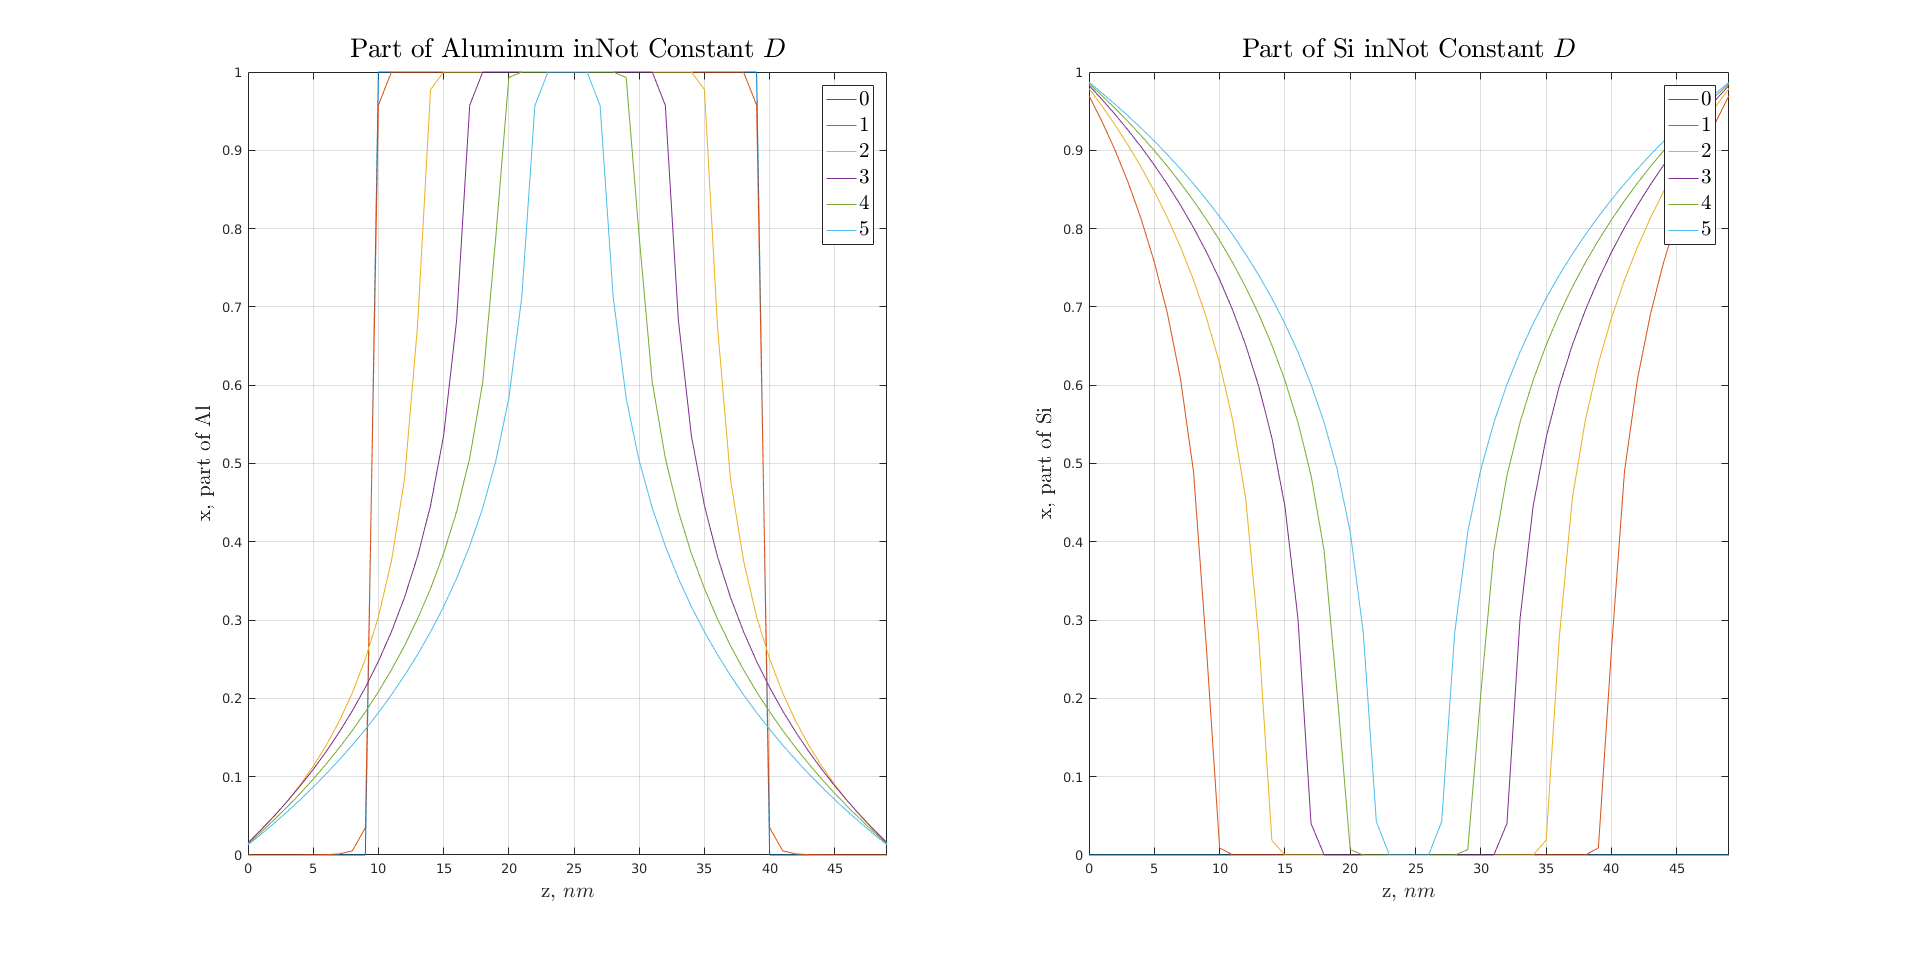
\includegraphics[width=0.9\linewidth]{assets/DSi}
	\caption{Диффузионное расплытие гетероструктуры $i$-$GaAs$/$i$-$AlAs$/$i$-$GaAs$ при $T = 430\,K$}
	\label{fig:DSi}
\end{figure}